\documentclass[a4paper,12pt]{article}
\usepackage[top = 3cm, bottom = 2cm, left = 3cm, right=2cm]{geometry}
\usepackage[utf8]{inputenc}
\usepackage{amsmath,amsfonts,amssymb}
\usepackage{float}
\usepackage{graphicx}
\usepackage[english]{babel}
\usepackage{indentfirst}
\usepackage{float}
\usepackage{textcomp}
\usepackage{gensymb}
\usepackage{subfigure}
\usepackage{enumerate}
\title{CDM Description - ARAM}

\begin{document}
	\maketitle
	\section{CDM Development}
	Knowing that the aparent solar diameter observed on the celestial vault is aproximately $0,5^{\circ}$, it was assumed, for each cylinder of sensor element, the value of $2^{\circ}$ as  FoV, Fiel of View. This value represents a detection region that covers 4 solar diameters. 
	
	The Figure \ref{Fig:MCD_1} represents the initial cylinder that comports a LDR. The calculations below were based on it. Remembering that R: LDR radius and L: the cylinder length.

\begin{figure}[htb] 
	\centering
	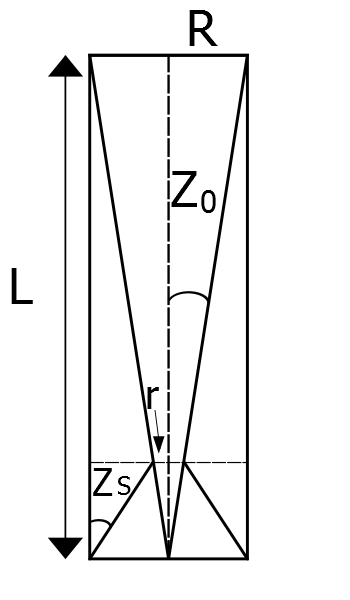
\includegraphics[scale=0.5]{img/MCD_1.jpg}
	\caption{First version of a cylinder to the sensors matrix.}
	\label{Fig:MCD_1}
\end{figure}

$$\frac{R}{L} = tan(Z_{0}) ; \,\,   R = \frac{D_{LDR}}{2}, Z_{0} = \frac{FoV}{2}$$
$$L = \frac{R}{tan(Z_{0})} \longrightarrow L = \frac{2}{tan(1^{o})}  \longrightarrow L \cong 115 mm$$ 


It was found that the length of the tube was too large relative to its diameter, this causes a problem in quality of the printed resistant plastic, therefore it was necessary to add the parameter $Z_{0}$ to the tube. This parameter not only changed the geometry of the cylinder into a conical trunk, but also enabled the preservation of the FoV of each cylinder as well as the reduce its length by approximately 50\% ,features that facilitate the 3D prototyping process and guarantee proportionality in the CDM dimensions.
	

$$Tan(Z_{s}) = \frac{(R-r)}{L_{new}}  \, ; \,  where: \, r= \,1mm \,e \, L_{new}= \, 60mm $$
$$Tan(Z_{s}) = \frac{(2-1)}{60}  \longrightarrow   Z_{s} = Tan^{-1}(0,0167) \therefore Z_{s} \cong 1^{\circ} $$

Once dimensioned each cylinder, another problem was found: having more than one sensor tracking the sun in the same time. This problem happens because the sun is located to millions of kilometers away from land, and in the first version of the matrix of sensors, the axes of the tubes were dimensioned parallel to each other, in other words, the cylinders point to the same region. The solution developed to correct this problem it was to create an angular difference between the axes, tilt them.Ensure the slope of pipes on a flat surface became quite complex, so it was  developed the CDM (Detection of Circular Matrix).

The CDM structure is composed of 25 tubes arranged  concentric circles in the surface of a spherical cap. The  calculated parameters below signify: tranversal radius section (X), center distance of the support sphere,theoretical, until the  CDM beggining (d), the arrow length (F), and the solid FoV of the matrix (FoV$_{S}$).
\begin{figure}[htb] 
	\centering
	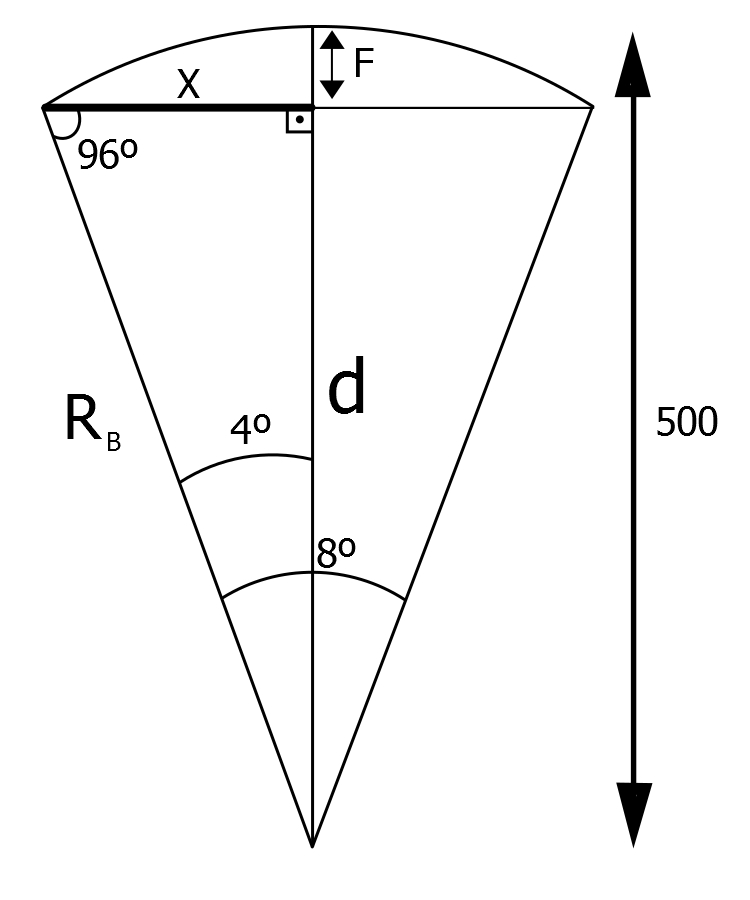
\includegraphics[scale=0.25]{img/MCD_2.jpg}
	\caption{MCD.}
\end{figure}
$$ \frac{X}{sin(4^{\circ})} = \frac{R_{B}}{sin(90^{\circ})}\longrightarrow X= \frac{R_{B}\times sin(4^{\circ})}{sin(90^{\circ})} \longrightarrow X=\frac{500\times 0,06975}{1} \therefore X=34,87mm $$
$$d = \sqrt{500^{2} - 34,87^{2}} \therefore d=498,78mm \, ;\, F=500-498,78 \therefore F=1,22mm $$
$$ A_{\bot } = \pi\times(34.87)^{2} \therefore A_{\bot } = 3.819,92mm^{2} $$ 
$$ FoV_{S} = \frac{A_{\bot }}{(R_{B})^{2}} \longrightarrow FoV_{S} =\frac{3.819,92}{500^{2}} \therefore FoV_{S} = 0,0153 \, strad$$ 
\newpage

Then it was calculated the distance between each tubes layer of the CDM, between centers (S), it was performed in the condition indicated by a single tube.
\begin{figure}[htb] 
	\centering
	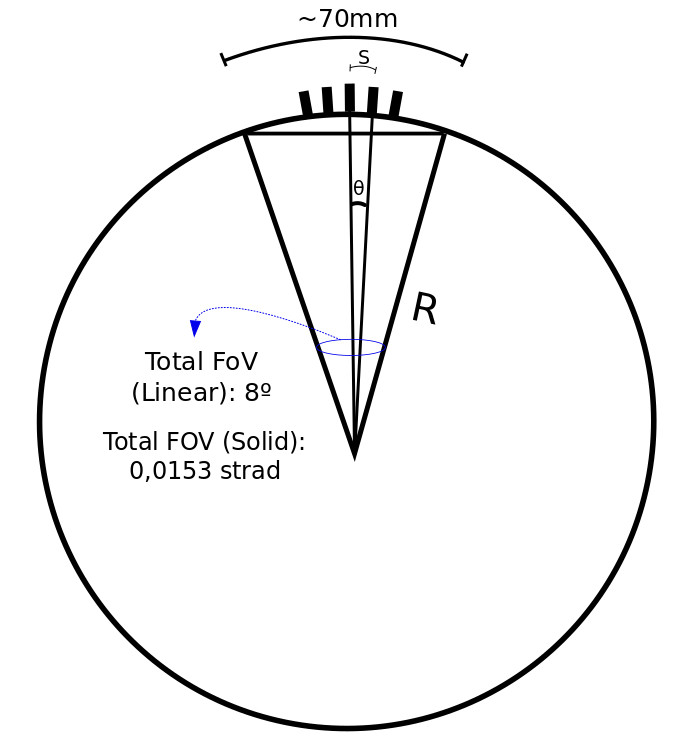
\includegraphics[scale=0.25]{img/MCD_3.jpg}
	\caption{Side cut of the CDM.}
\end{figure}

$$ \pi \longleftrightarrow 180^{\circ}$$
$$ X_{S} \longleftrightarrow 1^{\circ}$$
$$X_{S} = \frac{\pi}{180^{\circ}} \therefore X_{S} = 0,01745\, strad$$
$$\therefore \theta = 1^{\circ} = 0,01745 \,strad$$
$$S= R\times \theta \longleftrightarrow S= 500\times 0,01745 \therefore S=8,7mm $$

Finally, it was developed the CDM model in Creo Parametric software. In this step,
the geometry of each collimator element returned to be cylindrically, however, to ensure the
same functionality and FoV, each tube has a hole 1 mm. The figures 4.a,
4.b and 4.c represent the developed model.

\begin{figure}[h]
	
	\center
	\subfigure[ref1][]{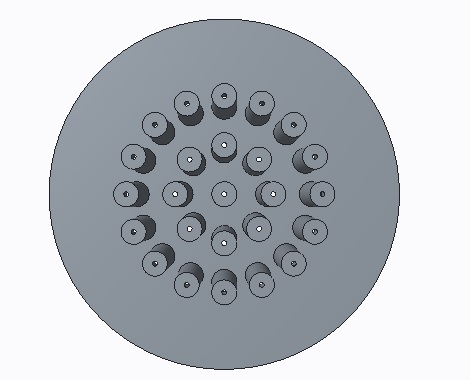
\includegraphics[width=4cm]{img/MCD_vista_de_cima.jpg}}
	\qquad
	\subfigure[ref2][]{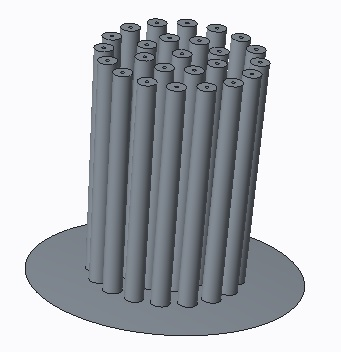
\includegraphics[width=4cm]{img/MCD_Lateral_esquerda.jpg}}
	\qquad
	\subfigure[ref2][]{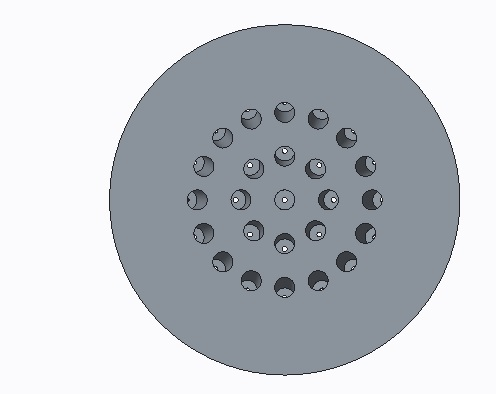
\includegraphics[width=4cm]{img/MCD_vista_de_baixo.jpg}}
	\caption{(a) Upper view. (b) Left side view. (c) Bottom view.}
	
	
\end{figure}
 \newpage
 \section{Algoritmo de apontamento fino}

Após realizar o apontamento grosso, por efemérides, um dos sensores da MCD detecta o sol. Em seguida o algoritmo de apontamento fino calcula a distância entre o sensor que encontrou o sol e o sensor central da MCD. Com auxílio do par de motores ortogonais, o algoritmo de detecção guia o apontamento sol para o sensor que se encontra no centro da matriz de sensores.

 O sensor central foi projetado para estar alinhado com o radiômetro em escala reduzida. Pode-se dizer que este algoritmo de apontamento fino faz com que o instrumento esteja apontando efetivamente para o sol, conduzindo  o eixo principal do instrumento até a posição aonde estava o eixo do cilindro que detectou o sol. As figuras abaixo ilustram o procedimento.
 \begin{figure}[h]
 	
 	\center
 	\subfigure[ref1][Comportamento antes do apontamento grosso.]{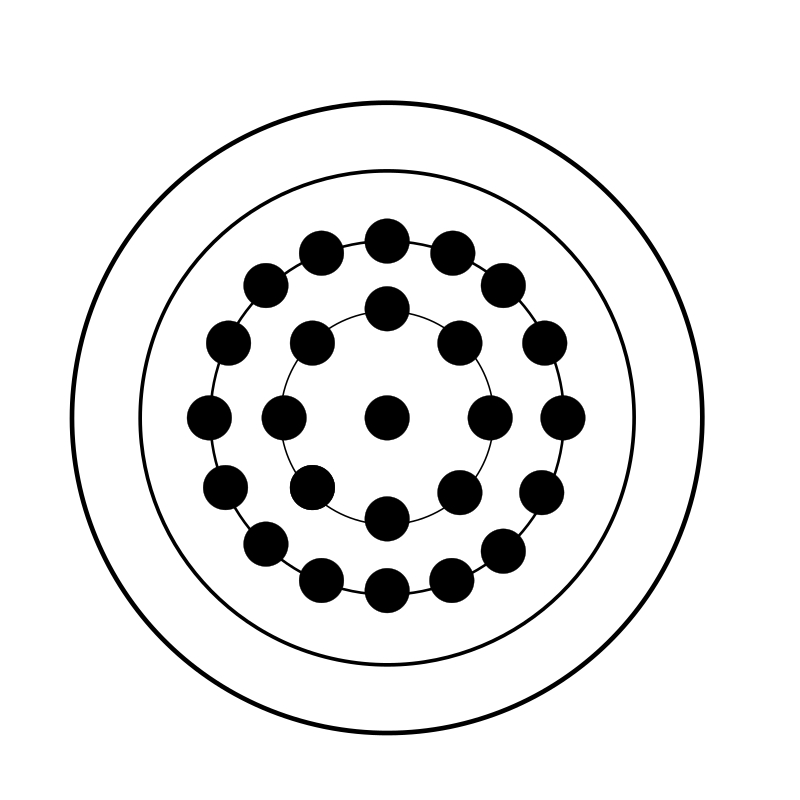
\includegraphics[width=4cm]{img/MCD_4.jpg}}
 	\qquad
 	\subfigure[ref2][Comportamento após o apontamento grosso.]{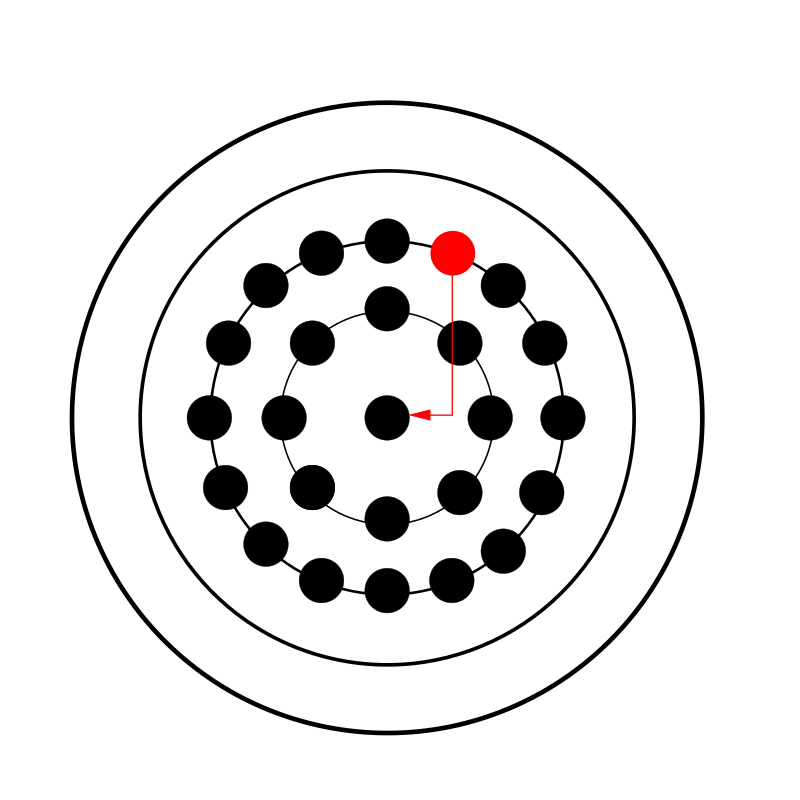
\includegraphics[width=4cm]{img/MCD_5.jpg}}
 	\qquad
 	\subfigure[ref2][Comportamento após apontamento fino.]{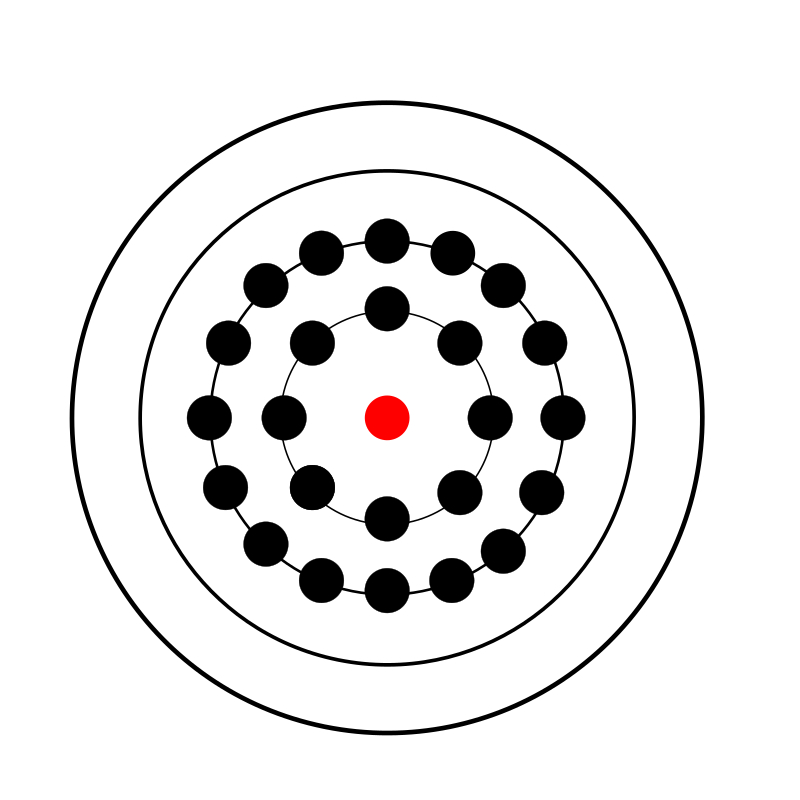
\includegraphics[width=4cm]{img/MCD_6.jpg}}
 	\caption{Etapas do algoritmo de apontamento fino.}
 	
 \end{figure}

\end{document}